% vim: set spell : spelllang=en_gb
\documentclass{beamer}
\author{Chiel Kooijman\\ Supervisor: Diederik Roijers}
\title{Dynamic priority broadcasting channels:\\a multi-objective planning problem}
\usepackage{graphicx,amsmath}
%\usepackage[round]{natbib}
\usetheme{boxes}
\usecolortheme[named=black]{structure}
\begin{document}
\frame{\titlepage}

%\frame{\frametitle{Table of contents}\tableofcontents}

\section{Introduction}
\begin{frame}{The broadcasting-channel problem}
	\begin{itemize}
		\item One Channel
		\item Multiple Agents
		\item Concrete time-steps
		\item Agent's buffer can contain a message or be empty
		\item Actions:
			\begin{itemize}
				\item Send (if buffer not empty)
				\item Do not send
			\end{itemize}
		\item Effects (and feedback):
			\begin{itemize}
				\item Success
				\item Collision
				\item Nothing sent
			\end{itemize}
	\end{itemize}
	\cite{ooi1996decentralized}
\end{frame}


\begin{frame}{Dynamic priority multi-objective planning}
	\begin{description}
		\item[\bf multi-objective:] Maximise throughput while preventing
			dominance of the channel by one or a few agents
			\cite{barrett2008learning}
		\item[\bf dynamic priority:] Change the priority of some messages or some
			agent at any time \cite{natarajan2005dynamic}
		\item[\bf planning:] Markov Decision Process (MDP): Dynamic programming
			where the optimal policy can be found by assigning rewards to states
			or state-action pairs \cite{hansen2004dynamic}
	\end{description}
\end{frame}

\begin{frame}{Dynamic optimal policy: Multidimensional reward}

	\begin{figure}
		\caption{Pareto-optimal set of solutions}
		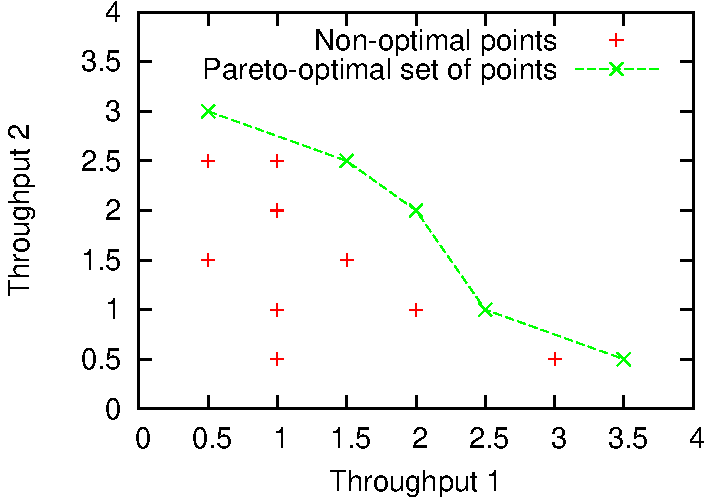
\includegraphics[scale=0.5]{pareto}
	   \label{fig:pareto}
	\end{figure}

	\begin{equation}
		\label{eq:pareto}
		\Big\{ V\, \Big| \, \forall V'[ V \neq V' \land \exists n [V_n > V'_n]] \Big\}
	\end{equation}
	\cite{vamplew2011empirical}
\end{frame}

\begin{frame}{Reward representation}

	\begin{tabular*}{\linewidth}{l|l}
	$\vec{r} = \begin{bmatrix}
		\mu\\
		\sigma\\
	\end{bmatrix}$ &
	$\vec{r} = \begin{bmatrix}
		t_1\\
		\vdots\\
		t_n\\
	\end{bmatrix}$\\
										& \\
		Always two-dimensional	& Prioritisation\\
										& \\
										& Permutations are redundant:\\
	\end{tabular*}
	\vspace{1cm}

	$f_{\vec{\theta}}(\vec{r})~\textrm{with}~\vec{r} = \begin{bmatrix}
		7\\
		3\\
	\end{bmatrix},~
	\vec{\theta} = \begin{bmatrix}
		w_1\\
		w_2\\
	\end{bmatrix}$
	=\\
	$ f_{\vec{\theta}}(\vec{r})~\textrm{with}~\vec{r} = \begin{bmatrix}
		3\\
		7\\
	\end{bmatrix},~
	\vec{\theta} = \begin{bmatrix}
		w_2\\
		w_1\\
	\end{bmatrix}$
\end{frame}

\begin{frame}{Improvements}
	\begin{itemize}
		\item Event horizon $\rightarrow$ No horizon (Discounted reward)
		\item 2 agents $\rightarrow$ Multiple agents
		\item	Planning $\rightarrow$ Learning
		\item MDP $\rightarrow$ (Dec)POMDP
	\end{itemize}

\end{frame}

	\bibliographystyle{apalike}
	\bibliography{../references}
\end{document}
